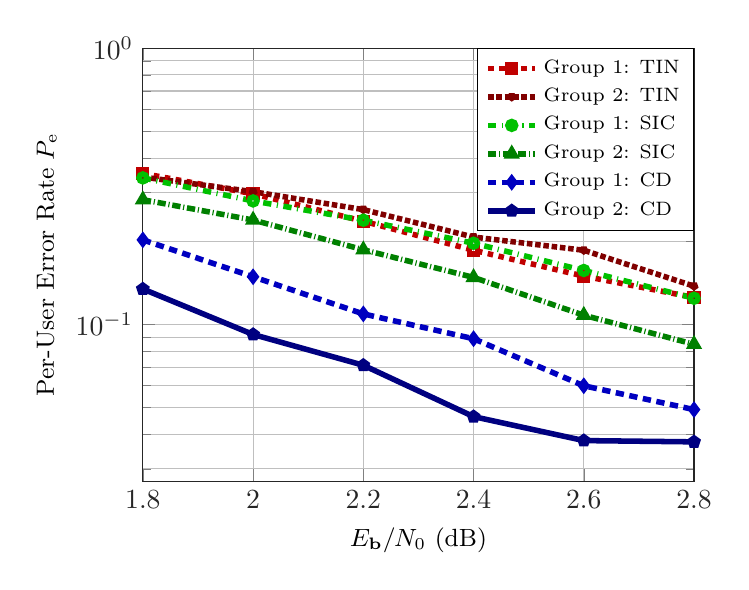
\begin{tikzpicture}
\definecolor{colorTIN2}{RGB}{128,0,0}
\definecolor{colorTIN1}{RGB}{192,0,0}
\definecolor{colorSIC2}{RGB}{0,128,0}
\definecolor{colorSIC1}{RGB}{0,192,0}
\definecolor{colorJD2}{RGB}{0,0,128}
\definecolor{colorJD1}{RGB}{0,0,192}
\begin{semilogyaxis}[
font=\small,
width=7cm,
height=5.5cm,
scale only axis,
every outer x axis line/.append style={white!15!black},
every x tick label/.append style={font=\color{white!15!black}},
xmin=1.8,
xmax=2.8,
xtick={1.8,2,2.2,2.4,...,2.8},
xlabel={$E_{\mathbf{b}}/N_0$ (dB)},
xmajorgrids,
xminorgrids,
every outer y axis line/.append style={white!15!black},
every y tick label/.append style={font=\color{white!15!black}},
% ymin=0,
ymax=1,
ytick={0.01, 0.1, 1.0},
ylabel={Per-User Error Rate $P_{\mathrm{e}}$},
ymajorgrids,
yminorgrids,
legend style={at={(1, 1)},anchor=north east,draw=black, fill=white, legend cell align=left,font=\scriptsize}
]
\addplot [color=colorTIN1, dotted,line width=2.0pt,mark size=1.4pt,mark=square,mark options={solid}]
  table[row sep=crcr]{
  1.8 0.352\\
  2 0.2972\\
  2.2 0.2364\\
  2.4 0.1856\\
  2.6 0.1496\\
  2.8 0.1252\\
};
\addlegendentry{Group 1: TIN};

\addplot [color=colorTIN2,densely dotted,line width=2.0pt,mark size=1.4pt,mark=star,mark options={solid}]
  table[row sep=crcr]{
  1.8 0.3416\\
  2 0.3024\\
  2.2 0.2604\\
  2.4 0.2072\\
  2.6 0.1856\\
  2.8 0.1376\\
};
\addlegendentry{Group 2: TIN};


\addplot [color=colorSIC1,dashdotted,line width=2.0pt,mark size=1.4pt,mark=o,mark options={solid}]
  table[row sep=crcr]{
  1.8 0.3392\\
  2 0.28\\
  2.2 0.2384\\
  2.4 0.1968\\
  2.6 0.1568\\
  2.8 0.1244\\
};
\addlegendentry{Group 1: SIC};

\addplot [color=colorSIC2,densely dashdotted,line width=2.0pt,mark size=1.4pt,mark=triangle,mark options={solid}]
  table[row sep=crcr]{
  1.8 0.2828\\
  2 0.2388\\
  2.2 0.1864\\
  2.4 0.148\\
  2.6 0.108\\
  2.8 0.0848\\
};
\addlegendentry{Group 2: SIC};


\addplot [color=colorJD1,densely dashed,line width=2.0pt,mark size=1.4pt,mark=diamond,mark options={solid}]
  table[row sep=crcr]{
  1.8 0.2024\\
  2 0.1488\\
  2.2 0.1092\\
  2.4 0.0888\\
  2.6 0.06\\
  2.8 0.0492\\
};
\addlegendentry{Group 1: CD};

\addplot [color=colorJD2,solid,line width=2.0pt,mark size=1.4pt,mark=pentagon,mark options={solid}]
  table[row sep=crcr]{
  1.8 0.1344\\
  2 0.092\\
  2.2 0.0712\\
  2.4 0.0464\\
  2.6 0.038\\
  2.8 0.0376\\
};
\addlegendentry{Group 2: CD};

% \addplot [color=colorTIN1, dashdotted,line width=2.0pt,mark size=1.4pt,mark=square,mark options={solid}]
%   table[row sep=crcr]{
%   1.8 0.3468\\ % 
%   2 0.2998\\%
%   2.2 0.2484\\%
%   2.4 0.1964\\%
%   2.6 0.1676\\%
%   2.8 0.1314\\%
% };
% \addlegendentry{TIN};

% \addplot [color=colorSIC2,densely dashdotted,line width=2.0pt,mark size=1.4pt,mark=triangle,mark options={solid}]
%   table[row sep=crcr]{
%   1.8 0.311\\
%   2 0.2594\\
%   2.2 0.2124\\
%   2.4 0.1724\\
%   2.6 0.1324\\
%   2.8 0.1046\\
% };
% \addlegendentry{SIC};

% \addplot [color=colorJD2,solid,line width=2.0pt,mark size=1.4pt,mark=pentagon,mark options={solid}]
%   table[row sep=crcr]{
%   1.8 0.1684\\
%   2 0.1204\\
%   2.2 0.0902\\
%   2.4 0.0676\\
%   2.6 0.049\\
%   2.8 0.0434\\
% };
% \addlegendentry{Coded Demixing};
\end{semilogyaxis}
\end{tikzpicture}